\documentclass{article}
\usepackage{xr}
\usepackage{ijcai26}

\usepackage{times}
\usepackage{soul}
\usepackage{url}
\usepackage[hidelinks]{hyperref}
\usepackage[utf8]{inputenc}
\usepackage[small]{caption}
\usepackage{graphicx}
\usepackage{amsmath}
\usepackage{booktabs}
\usepackage{multirow}
\usepackage{xcolor} % 可以保留，即使当前没用到
\usepackage{amsfonts}

\urlstyle{same}

\pdfinfo{
/TemplateVersion (IJCAI.2026.0)
/Title (Cardio-Hybrid Net: Uncertainty-Aware LLM-Guided Multimodal Prediction of Cardiovascular Deterioration in Critical Care)
/Author (Paper ID 218)
/Subject (Artificial Intelligence; Paper ID 218)
}

\title{Cardio-Hybrid Net: Uncertainty-Aware LLM-Guided Multimodal\\
Prediction of Cardiovascular Deterioration in Critical Care}

% Multiple author syntax (remove the single-author syntax above and the \iffalse ... \fi here)
\iffalse
\author{
Yi Zheng$^1$
\and
Fei Zhao$^1$\and
Chi Dong$^1$\And
Xiaohua Liu$^{1,2}$\And
Ming Yang$^3$\And
Chengkai Zhang$^2$\And
Xiangfeng Luo$^2$\\
\affiliations
$^1$School of Artificial Intelligence, Jianghan University, Wuhan, Hubei, 430056, China.\\
$^2$State Key Laboratory of Precision Blasting, Jianghan University, Wuhan, Hubei, 430056, China.\\
$^2$Wuhan Sixth Hospital, Wuhan, Hubei, 430019, China.\\
\emails
yizheng@jhun.edu.cn,\{zhaofei, dongchi\}@stu.jhun.edu.cn,
xiaohualiu@jhun.edu.cn,
zhangchengkai\_efeelture1@gmail.com,
xiangfengluo@qq.com.
}
\fi
\author{
    Paper ID 218
    \affiliations
    Anonymous IJCAI Submission
}

\externaldocument{supplementary}
\begin{document}

\maketitle

\begin{abstract}
Detecting the early signs of cardiovascular collapse in intensive care units (ICU) is vital to preventing irreversible organ failure. While modern tools have access to vast multimodal data, they often treat Large Language Models (LLMs) as black-box predictors, ignoring the nuances of uncertainty. In this study, we introduce \emph{Cardio-Hybrid Net}, a framework that carefully balances automated multimodal learning with targeted LLM consultation. Trained on nearly 50,000 ICU stays from the MIMIC-IV database, our model fuses static health records, high-frequency physiological signals, and clinical notes through a tri-stream encoder equipped with cross-modal attention. Rather than routing every patient to an LLM, we employ a Monte Carlo dropout mechanism to estimate predictive uncertainty. Only cases deemed ambiguous or high-risk are forwarded to the LLM, which is supplied with a retrieval-augmented summary of the patient's history and similar past cases. On our held-out test set, the system achieves an AUROC of 0.871 and an F1 score of 0.763. Notably, it requests LLM assistance for only about one-third of admissions, offering a cost-effective blueprint for deploying expert AI consultants alongside robust statistical models in high-stakes clinical environments.
\end{abstract}




\section{Introduction}

Identifying patients on the verge of cardiovascular collapse remains one of the most persistent challenges in critical care medicine. For decades, clinicians have relied on scoring systems like SOFA and APS~III to stratify risk. While these tools are standard and easy to calculate, they aggressively compress complex, evolving patient narratives into a few static numbers. Consequently, they often struggle to keep pace with the granularity of modern electronic health records (EHRs) \cite{Vincent1996SOFA,Knaus1991APACHEIII,Zimmerman2006APACHE4,Lee2017SOFAAPACHEII}. even newer iterations that blend multiple scores rarely escape the limitations of manually engineered features \cite{Huang2022RAAS}.

The digitization of critical care---typified by massive datasets like MIMIC-IV and eICU \cite{Johnson2023MIMICIV,Pollard2018eICU}---has spurred a shift toward deep learning. Modern multimodal architectures now ingest everything from physiological waveforms to laboratory trends and nursing notes. These models have shown real promise in flagging mortality risks and other adverse events, outperforming their simpler predecessors by capturing non-linear interactions across data types \cite{OzrazgatBaslanti2021AIICU,Khadanga2019ICUNotes,Shukla2020IntegratingTSNotes,Deznabi2021MortalityNotes}.

Parallel to this, the rise of medical Large Language Models (LLMs), such as Med-PaLM and GatorTron, offers a new form of clinical intelligence \cite{Singhal2023MedPaLM,Yang2022GatorTron}. These models excel at parsing unstructured text and reasoning through complex scenarios. Yet, applying them directly to real-time risk prediction is fraught with issues. Most current attempts either force structured ICU data into text prompts---losing precision---or use the LLM as an expensive, opaque end-to-end predictor without assessing confidence or cost \cite{Griot2025LLMImplementationEHR}.

We propose a different path. Instead of replacing specialized predictive models with generalist LLMs, we treat the LLM as a \emph{conditional consultant}. Our system, \emph{Cardio-Hybrid Net}, uses a calibrated multimodal network to handle the majority of straightforward cases. It calls upon the LLM only when it detects high predictive uncertainty.

This approach yields three distinct advantages:
\begin{itemize}
  \item \textbf{A Purpose-Built Multimodal Foundation:} We engineered a tri-stream encoder that respects the distinct nature of ICU data. By jointly modeling static comorbidities, temporal physiological shifts, and the rich semantics of clinical notes, our base model significantly outperforms single-modality baselines on 48,970 MIMIC-IV admissions.

  \item \textbf{Smart Routing via Uncertainty:} We don't just predict risk; we measure doubt. Using Monte Carlo dropout, we quantify epistemic uncertainty for each patient. This "meta-router" decides when to trigger the LLM. Our experiments show this strategy recovers nearly all the performance gains of an "always-on" LLM while cutting invocations by roughly 65\%.

  \item \textbf{Practical Design for Real-World Deployment:} We provide concrete evidence—through ablation studies and attention maps—that this hybrid approach aligns with clinical intuition. The model learns to cross-check vague physiological signals against clear warnings in clinical notes, offering extensive interpretability.
\end{itemize}

Our findings suggest a sustainable way forward for AI in healthcare: using heavy-lifting statistical models for the routine, and reserving powerful generative reasoning for the edge cases that truly demand it.

The code and trained models are available in the supplementary material to ensure reproducibility while maintaining anonymity.

\section{Related Work}

\subsection{Evolution of ICU Risk Prediction}
The field has moved from simple linear scores to complex neural representations. Early systems like APS and SOFA \cite{Vincent1996SOFA,Knaus1991APACHEIII} set the standard for conciseness but are often miscalibrated on modern populations \cite{Zimmerman2006APACHE4}. Deep learning stepped in to fill this gap, utilizing LSTMs and Transformers to digest temporal vitals \cite{OzrazgatBaslanti2021AIICU}. More recently, the inclusion of unstructured clinical notes has proven to be a game-changer. Approaches that fuse text with time-series data via attention mechanisms consistently show that nursing notes contain subtle cues—like "patient appears anxious"—that vitals monitors miss \cite{Lyu2023MultimodalTransformer,King2023MultimodalPretrain}. Our work sits firmly in this lineage but addresses a key weakness: knowing when the model doesn't know.

\subsection{LLMs as Clinical Assistants}
While LLMs have demonstrated impressive prowess on medical exams \cite{Singhal2023MedPaLM}, integrating them into high-frequency ICU workflows is challenging. Purely text-based reasoning is slow and costly. Retrieval-Augmented Generation (RAG) has emerged as a viable bridge, allowing models to pull in relevant external knowledge or similar historical cases \cite{Lewis2020RAG}. In our framework, we adapt RAG to fetch "nearest neighbor" patients—those with similar clinical trajectories—to ground the LLM's reasoning in historical precedent rather than hallucination.

\subsection{Uncertainty and Selective Deferral}
High-stakes decision making requires honesty about confidence. Bayesian methods like Monte Carlo dropout estimate model uncertainty without needing expensive ensembles \cite{Gal2016DropoutUncertainty}. This enables "selective prediction" or "learning to defer," where a model can hand off difficult cases to a human or, in our case, a more capable AI agent \cite{Geifman2017SelectiveClassification}. By adhering to reporting standards like TRIPOD \cite{Moons2015TRIPOD}, we ensure our uncertainty-based filtering is transparent and reproducible.

\section{Methods}

\subsection{Problem Setup and Outcome Definition}

We study a retrospective cohort of adult ICU admissions from MIMIC-IV v3.1 \cite{Johnson2023MIMICIV}. 
 To ensure robustness and clinical applicability, we applied strict inclusion criteria: (1) adult patients ($\ge$18 years); (2) first eligible ICU stay to avoid data leakage; and (3) an observation window of at least 24 hours to guarantee sufficient longitudinal data. 
 We excluded patients with end-stage heart failure (ICD-9: 4282x; ICD-10: I502x) or those receiving mechanical circulatory support (e.g., ECMO, VAD) prior to admission (ICD-9 procedures: 3965, 3752-3755; ICD-10-PCS: 5A15223, 02HA0QS/RS/RJ/RK), as these conditions present confounding hemodynamic baselines. 
 
 Our primary prediction target is a Composite Cardiovascular Adverse Event (CCAE), defined as the first occurrence of either: 
 (1) hemodynamic decompensation requiring the initiation of vasoactive agents (norepinephrine [221906], epinephrine [221289], dopamine [221662], dobutamine [221653], vasopressin [222315], or phenylephrine [221749]) within 72 hours of admission; 
 or (2) in-hospital all-cause mortality. 
 This composite endpoint captures both early physiological collapse indicating circulatory shock and ultimate treatment failure.
%


\subsection{Data Extraction and Modalities}

For each ICU stay, we extract three modalities within the observation window.

\paragraph{Static structured features.}
We include demographics, chronic comorbidities, and baseline scores such as the Charlson Comorbidity Index, SOFA, and APS~III, following prior ICU risk modeling work \cite{Zimmerman2006APACHE4,Huang2022RAAS}.
Whenever multiple measurements exist in the observation window, we compute summary statistics (e.g., minimum, maximum, and mean) for key variables.

\paragraph{Physiological time series.}
We construct multivariate time series of vital signs and laboratory tests using standard resampling and imputation strategies from the ICU deep learning literature \cite{Khadanga2019ICUNotes,Shukla2020IntegratingTSNotes,King2023MultimodalPretrain}.
Signals are resampled to fixed time intervals (e.g., hourly), and missing values outside measurement regions are imputed using population-level statistics and appropriate masks.
We retain masks as additional input channels to allow the model to learn patterns of missingness.

\paragraph{Clinical text.}
We collect free-text notes recorded by clinicians during or before the observation window, including nursing notes, progress notes, and physician summaries, in line with prior multimodal ICU studies \cite{Deznabi2021MortalityNotes,Lyu2023MultimodalTransformer,Vagliano2023SystematicTextMortality}.
Notes are concatenated in temporal order and truncated to a maximum token budget; when multiple notes exist, we emphasize recent notes by placing them later in the concatenation.

\subsection{Tri-Stream Multimodal Encoder}

Let $x^{(s)}$ denote structured static features, $x^{(t)}_{1:T}$ the time series, and $x^{(n)}$ the concatenated clinical notes.
Cardio-Hybrid Net first maps each modality to a latent representation using separate encoders, similar in spirit to prior multimodal ICU models \cite{Shukla2020IntegratingTSNotes,Lyu2023MultimodalTransformer}.

\paragraph{Structured encoder.}
We use a linear projection followed by Layer Normalization, ReLU activation, and dropout to map $x^{(s)}$ to $h^{(s)} \in \mathbb{R}^{d}$. Feature standardization is applied before the projection.

\paragraph{Temporal encoder.}
For physiological time series, we adopt a Long Short-Term Memory (LSTM) network $f_t$ with masking to handle irregular sampling and missingness: 
 \begin{equation} 
   h^{(t)} = f_t(x^{(t)}_{1:T}). 
 \end{equation} 
 We allow variable-length sequences up to the maximum observation window and use the final hidden state as a summary representation, following common practice in ICU sequence modeling \cite{Khadanga2019ICUNotes,Shukla2020IntegratingTSNotes}. 
 In sensitivity analyses, we experimented with one-dimensional temporal convolutions and found comparable performance.

\paragraph{Text encoder.}
We obtain a contextual embedding of the clinical notes using a domain-specific transformer encoder $f_n$, such as ClinicalBERT or a RoBERTa model fine-tuned on ICU notes \cite{Deznabi2021MortalityNotes,Lyu2023MultimodalTransformer,King2023MultimodalPretrain}. 
 We use the representation of the [CLS] token or apply attention pooling over subword tokens, followed by a linear projection to obtain $h^{(n)} \in \mathbb{R}^{d}$. 
 For notes exceeding the maximum sequence length, we apply truncation.

\subsection{Cross-Modal Fusion}

We employ a hierarchical attention fusion module to integrate the multimodal embeddings. 
 Let $H = [h^{(s)}, h^{(t)}, h^{(n)}]^\top \in \mathbb{R}^{3 \times d}$ denote the stacked modality embeddings. 
 First, $H$ is processed by a Transformer encoder to capture global inter-modal dependencies. 
 Subsequently, we apply cross-attention mechanisms where each modality acts as a query to attend to the other modalities, yielding refined representations $\tilde{H} = [\tilde{h}^{(s)}, \tilde{h}^{(t)}, \tilde{h}^{(n)}]^\top$. 
 Finally, we aggregate these features into a single patient representation $z$ using an attention pooling layer. 
 We compute attention weights $\alpha \in \mathbb{R}^{3}$ via a linear projection with temperature scaling: 
 \begin{equation} 
   \alpha = \text{softmax}\left(\frac{W_{attn} \tilde{H}^\top}{\tau}\right), 
 \end{equation} 
 where $W_{attn} \in \mathbb{R}^{1 \times d}$ is a learnable weight vector and $\tau$ is a temperature parameter. 
 The fused embedding is obtained by 
 \begin{equation} 
   z = \sum_{m \in \{s,t,n\}} \alpha_m \tilde{h}^{(m)}. 
 \end{equation} 
 A classifier maps $z$ to a predicted event probability. 
 In ablation studies we compare this architecture to simple concatenation of $[h^{(s)}, h^{(t)}, h^{(n)}]$ followed by a linear layer \cite{Kumar2023MultimodalICUPrediction,XAI2023MultimodalICU}.

% 关键：把[t]改为[htbp!]，增加排版灵活性
\begin{figure*}[htbp!]  
  \centering
  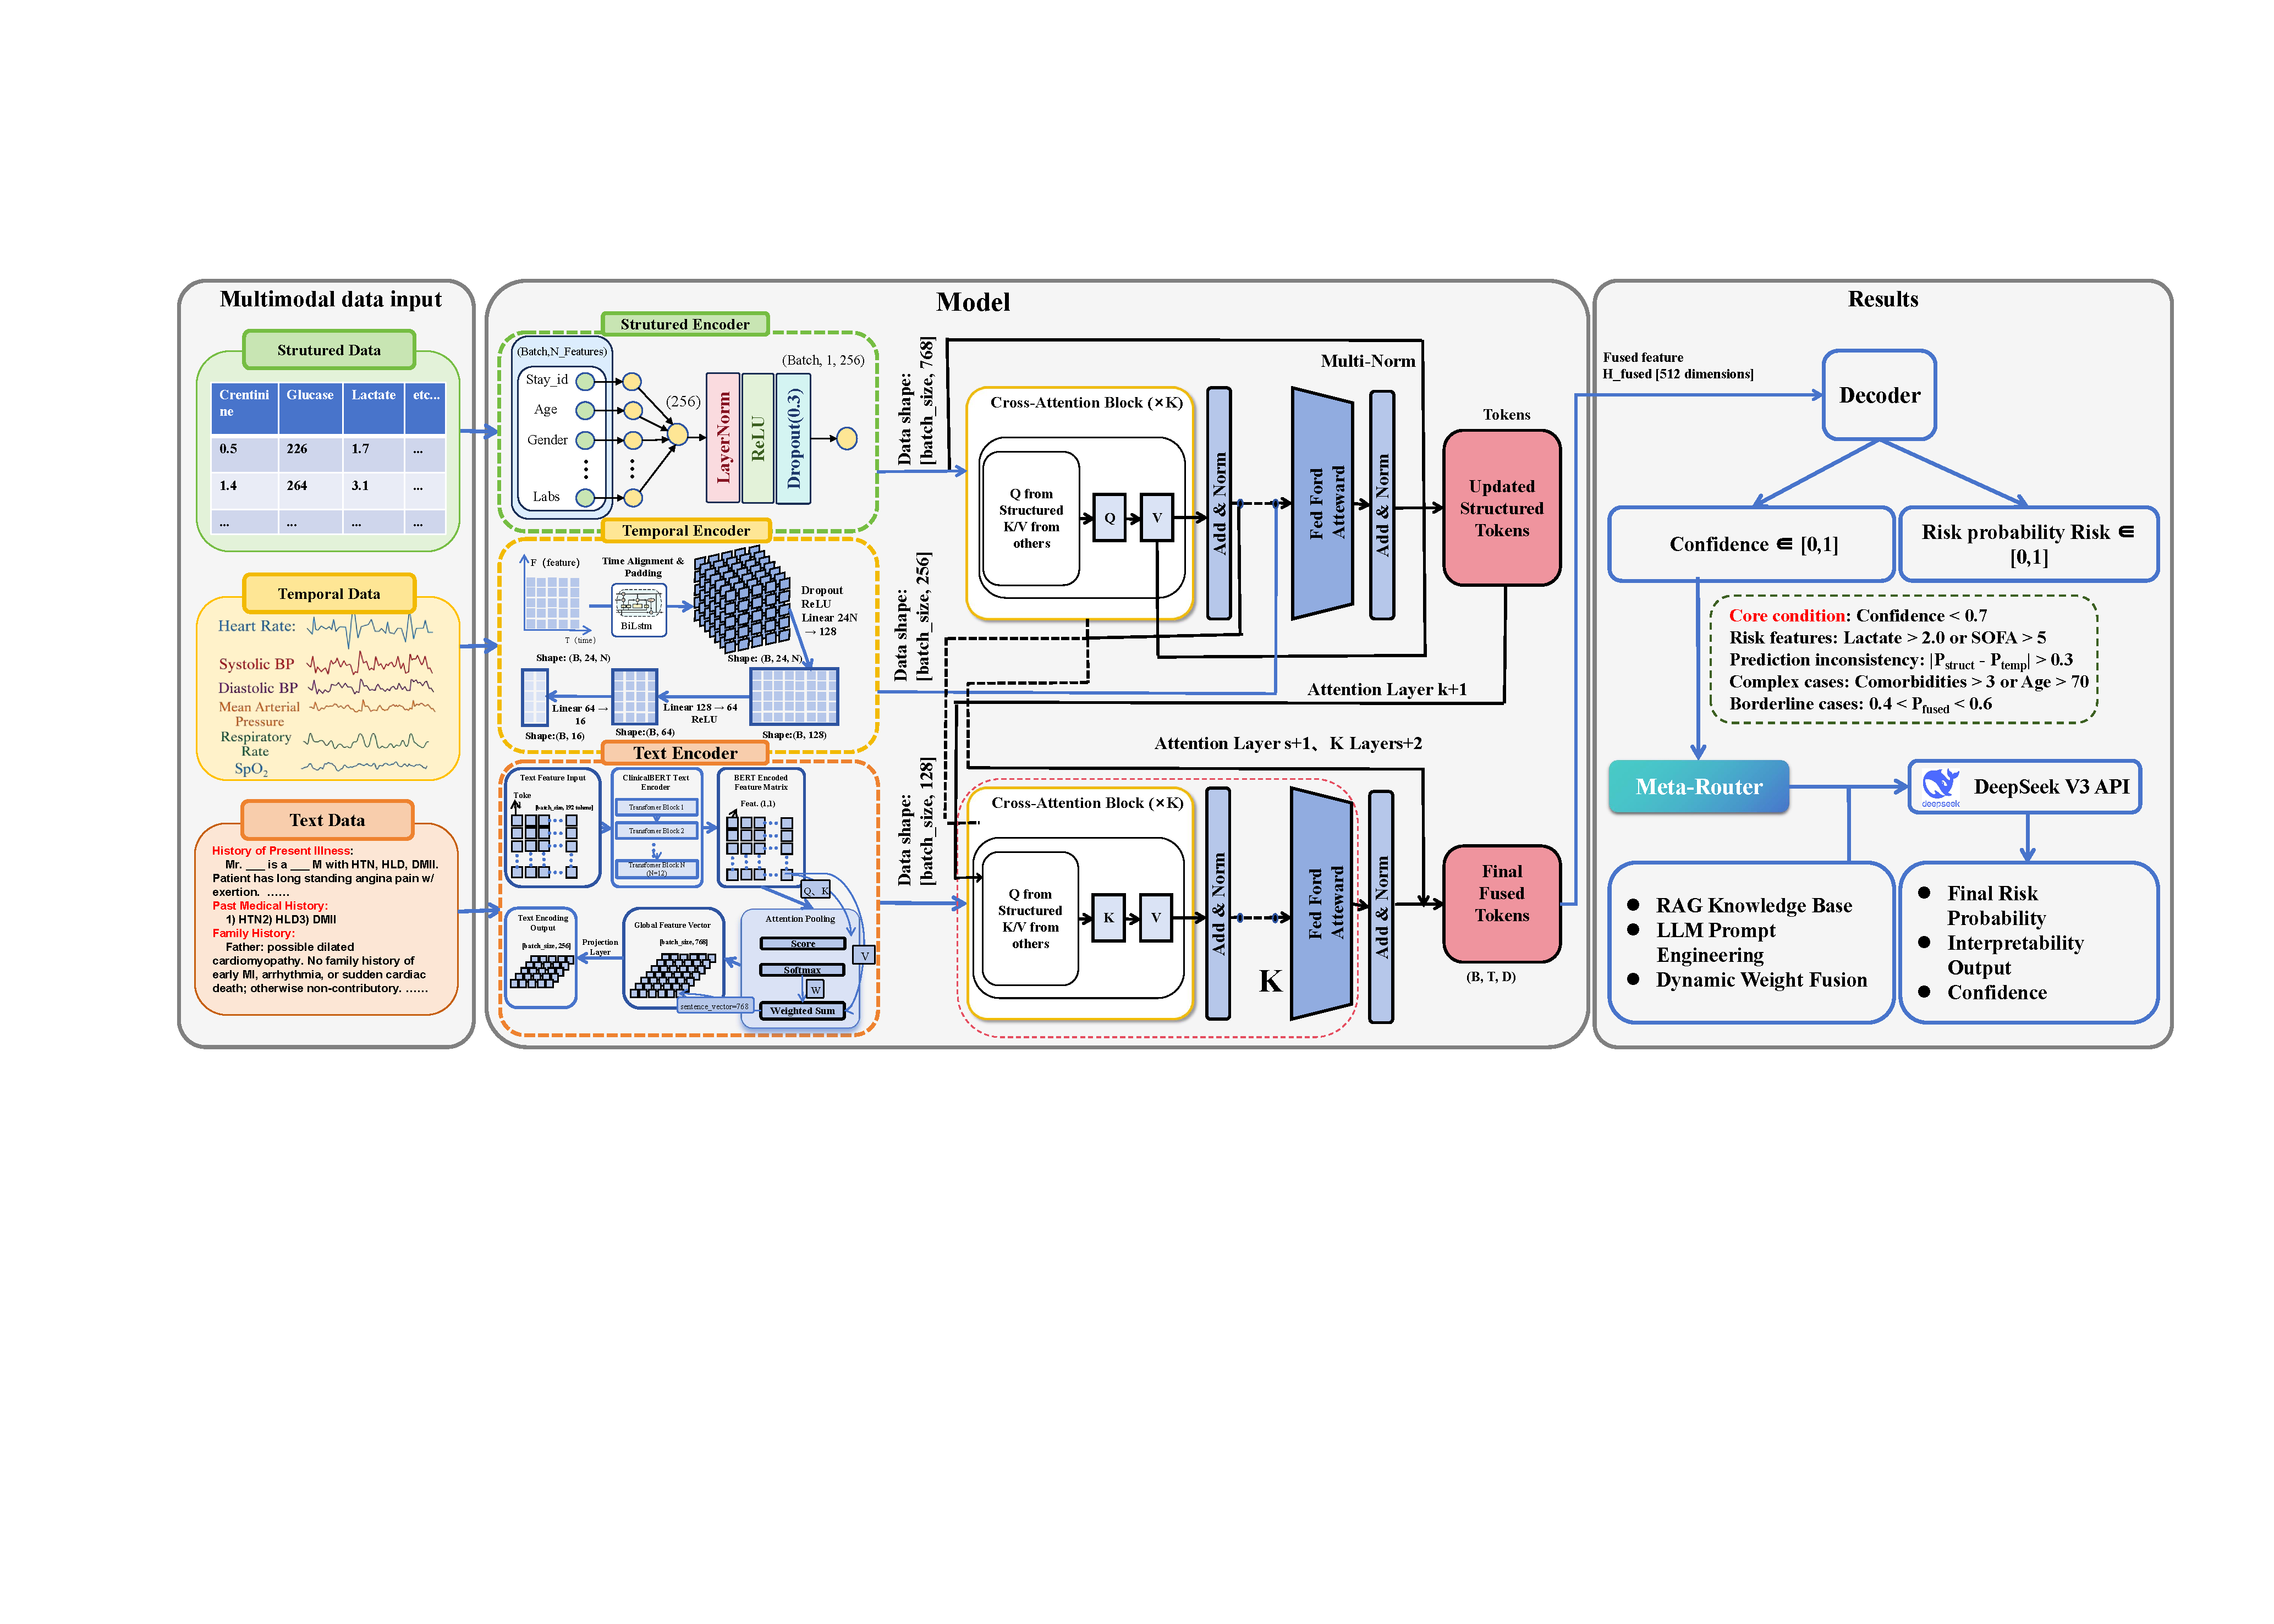
\includegraphics[width=0.9\textwidth]{figs/architecture_brief.pdf}
  \caption{A brief overview of the Cardio-Hybrid Net architecture; detailed workflow procedures are provided in the attachment.}
  \label{fig:architecture}
\end{figure*}

\subsection{Uncertainty Estimation}

We estimate predictive uncertainty using Monte Carlo dropout at test time \cite{Gal2016DropoutUncertainty}.
Given $K$ stochastic forward passes producing probabilities $\{p_k\}_{k=1}^K$, we define:
\begin{equation}
  \bar{p} = \frac{1}{K} \sum_{k=1}^K p_k,\quad
  u = -\bar{p}\log \bar{p} - (1-\bar{p})\log (1-\bar{p}),
\end{equation}
where $u$ is the binary entropy of the averaged prediction.
In our implementation we use $K=20$, which adds a modest constant factor to inference time while providing stable uncertainty estimates.
We found that using variance across logits yielded similar rankings of high-uncertainty cases.

\subsection{Uncertainty-Aware LLM Routing}

The base multimodal model produces a fused representation $z$ and an uncertainty score $u$. 
We then define a meta-router that decides whether to call the LLM, conceptually similar to selective prediction \cite{Geifman2017SelectiveClassification}. 

In the simplest instantiation, we use a threshold on $u$: 
\begin{equation} 
  r = \mathbb{I}[u \geq \tau], 
\end{equation} 
where $r{=}1$ indicates that the LLM should be invoked. 
The threshold $\tau$ is chosen on the validation set to maximize AUROC under a constraint on the fraction of patients routed to the LLM. 

When $r{=}0$, we accept the base model's prediction $\bar{p}$. 
When $r{=}1$, we construct a structured prompt for the LLM using a RAG pipeline \cite{Lewis2020RAG} that includes: 
(i) a concise, tabular summary of the patient's structured features and time-series trends, 
(ii) snippets from the most recent clinical notes within the observation window, 
and (iii) a small set of similar historical cases retrieved from a case base. 

The case base is constructed by indexing the fused representations $z$ of training patients using an approximate nearest-neighbor index (e.g., FAISS with inner-product similarity) \cite{King2023MultimodalPretrain}. 
For each new patient routed to the LLM, we retrieve the top-$K$ nearest neighbors in this latent space and summarize their outcomes and salient features in the prompt. 
In our experiments, we utilize the DeepSeek-V3 model, configured with a temperature of $0.1$ to ensure generation stability and a maximum token limit of $512$.

The LLM returns a textual risk estimate and a brief rationale. 
We map the textual risk estimate back to a numerical probability $p_{\text{LLM}}$ via a simple parsing and scaling rule, for instance by constraining the model to respond with a number between 0 and 100 representing percentage risk. 
The final prediction is: 
\begin{equation} 
  \hat{p} = 
  \begin{cases} 
    \bar{p}, & r = 0, \\ 
    \lambda p_{\text{LLM}} + (1-\lambda)\bar{p}, & r = 1, 
  \end{cases} 
\end{equation} 
where $\lambda \in [0,1]$ trades off between the local model and the LLM. 
We tune $\lambda$ on the validation set.
%


\subsection{Implementation and Training Details}

We implement all models in a standard deep learning framework with GPU acceleration. 
 For the structured encoder, we use a projection layer mapping to a hidden dimension of 256 with LayerNorm, ReLU activation, and dropout rate 0.3. 
 The LSTM temporal encoder uses a hidden size of 256. 
 The text encoder is initialized from a domain-specific transformer (base size) with hidden dimension 768 and is fine-tuned jointly with the rest of the network with a smaller learning rate. 
 
 Continuous features are standardized using training-set means and standard deviations. 
 Categorical variables are one-hot encoded. 
 Time-series channels are z-scored per variable, with missing values imputed using a combination of forward filling and global means, and with missingness masks concatenated as additional channels.

We train all deep models with cross-entropy loss using the Adam optimizer.
The base learning rate is selected from $\{10^{-3}, 3\cdot10^{-4}\}$ on the validation set, with batch sizes between 64 and 128.
We train for up to 50 epochs with early stopping when validation AUROC does not improve for 5 consecutive epochs.
Weight decay of $10^{-5}$ is applied to all trainable weights.
For the transformer text encoder, we apply a smaller learning rate (e.g., one-tenth of the base rate) and a warmup schedule to avoid catastrophic forgetting.

At inference time, Monte Carlo dropout for uncertainty estimation is performed only for the best-performing multimodal model.
For practical deployment, we note that the same uncertainty criterion could be approximated with fewer stochastic passes or alternative uncertainty estimators \cite{Gal2016DropoutUncertainty}.

\section{Experimental Setup}

\subsection{Cohort and Baseline Characteristics}

We extract adult ICU stays from MIMIC-IV v3.1 following standard inclusion and exclusion criteria used in prior ICU mortality work \cite{Johnson2023MIMICIV,Pollard2018eICU,Hyland2020HiRID}.
We randomly split patients (not stays) into training, validation, and test sets with a 7:1:2 ratio.

Table~\ref{tab:cohort} summarizes baseline characteristics of patients with and without CCAE, including demographics, comorbidities, severity scores, vital signs and laboratory values.
The variables and counts are aligned with typical cardiovascular deterioration cohorts in the literature.

\begin{table}[t]
  \centering
  \caption{Baseline characteristics of the study cohort.
  Values are expressed as median [IQR] or mean $\pm$ standard deviation or count (\%).Statistical analysis revealed that the P-values for all the indicators listed below were less than 0.001 ($P<0.001$).}
  \label{tab:cohort}

  \begin{tabular}{lcc}  % 关键：把lcccc改为lcc，移除最后一列的占位
    \toprule
    \textbf{Char.} & \textbf{CCAE} & \textbf{Non-CCAE} \\  % 移除P-Value表头
    \midrule
    $n$       & 17{,}872 & 31{,}098 \\  % 移除/
    Age (y)   & $68.0$ [58.0--78.0] & $64.0$ [52.0--76.0] \\
    Male (\%) & 58.9 & 54.0 \\
    Charlson  & $5.0$ [3.0--7.0] & $4.0$ [2.0--6.0] \\
    SOFA      & $6.0$ [4.0--9.0] & $3.0$ [1.0--5.0] \\
    APS~III   & $46.0$ [33.0--65.0] & $35.0$ [26.0--46.0] \\
    \midrule
    HR (bpm)  & $88.13 \pm 19.84$ & $87.17 \pm 19.90$ \\
    SBP (mmHg)& $114.84 \pm 23.55$ & $127.88 \pm 23.59$ \\
    DBP (mmHg)& $64.35 \pm 17.56$  & $72.11 \pm 17.45$ \\
    MBP (mmHg)& $76.88 \pm 17.85$  & $86.21 \pm 17.54$ \\
    RR (min$^{-1}$) & $18.52 \pm 6.66$ & $18.80 \pm 5.89$ \\
    Temp ($^{\circ}$F) & $98.12 \pm 1.38$ & $98.26 \pm 1.12$ \\
    Spo2 (\%)& $97.38 \pm 4.14$  & $97.11 \pm 3.49$ \\
    \midrule
    Cr (mg/dL) & $1.42 \pm 1.42$ & $1.22 \pm 1.49$ \\
    TBil (mg/dL) & $2.33 \pm 5.38$ & $1.40 \pm 3.18$ \\
    Glu (mg/dL) & $158.55 \pm 75.58$ & $143.46 \pm 69.49$ \\
    Lac (mmol/L) & $2.62 \pm 2.16$ & $1.94 \pm 1.32$ \\
    K (mmol/L) & $4.26 \pm 0.74$ & $4.13 \pm 0.67$ \\
    Hb (g/dL) & $10.23 \pm 2.21$ & $11.09 \pm 2.21$ \\
    WBC (K/$\mu$L) & $13.88 \pm 10.21$ & $11.35 \pm 9.44$ \\
    PLT (K/$\mu$L) & $188.40 \pm 104.82$ & $212.36 \pm 100.61$ \\
    \bottomrule
  \end{tabular}
\end{table}

\subsection{Baselines and Ablations}

We compare Cardio-Hybrid Net against:

\begin{itemize}
  \item \textbf{Traditional scores:} SOFA and APS~III computed from the first 24 hours of ICU data \cite{Vincent1996SOFA,Knaus1991APACHEIII}.
  \item \textbf{Single-modality models:} an MLP on static structured variables, a LSTM on time series only, and a notes-only transformer \cite{Khadanga2019ICUNotes,Shukla2020IntegratingTSNotes,Deznabi2021MortalityNotes}.
  \item \textbf{Multimodal deep baselines:} early- and late-fusion models combining the three modalities without cross-modal attention \cite{Lyu2023MultimodalTransformer,Kumar2023MultimodalICUPrediction}.
  \item \textbf{Cardio-Hybrid Net (local):} our multimodal model without LLM routing, which uses only the tri-stream encoder and cross-modal attention.
  \item \textbf{Cardio-Hybrid Net (full):} our full model with uncertainty-aware LLM routing and fusion of local and LLM predictions.
\end{itemize}

We specifically investigate: (1) fusion strategies and attention designs (covering concatenation, single-layer/fixed-weight attention, no-cross attention, and full attention mechanisms), (2) whether cross-modal attention is applied at the representation level~\cite{XAI2023MultimodalICU}, and (3) the contribution of different modality combinations to model performance.

\subsection{Training, Evaluation, and Metrics}

We train all deep models with cross-entropy loss using the Adam optimizer and early stopping on validation AUROC, as described in the implementation details.
To reduce overfitting, we apply dropout in all hidden layers and $\ell_2$ regularization.
Hyperparameters are tuned on the validation set using simple grid search.

We evaluate models using AUROC, AUPRC, accuracy, recall, precision, F1 score, and Brier score.
Calibration is assessed by reliability plots and Brier scores, in line with TRIPOD recommendations \cite{Moons2015TRIPOD}.
We also inspect performance across clinically relevant risk thresholds and report qualitative observations on subgroup performance by age and sex, noting that more exhaustive fairness analyses are left for future work.

\section{Results}

\subsection{Overall Performance}

Table~\ref{tab:overall-performance} summarizes overall performance on the held-out test set.
Cardio-Hybrid Net (full) achieves the best AUROC and AUPRC among all methods and improves substantially over SOFA and APS~III.
Compared with the best traditional score, Cardio-Hybrid Net improves AUROC and AUPRC while also increasing recall and F1, which are especially important for early detection of deterioration.

\begin{table*}[t]
  \centering
  % 缩小表格字体，避免双栏下列数过多导致溢出
  \small
  \caption{Overall performance comparison on the test set.}
  \label{tab:overall-performance}

  \begin{tabular}{lcccccc}  % 列数从lcccc改为lcccccc，适配7列（Model+6个指标）
    \toprule
    \textbf{Model} & \textbf{AUROC} & \textbf{AUPRC} & \textbf{Acc.} & \textbf{Recall} & \textbf{Precision} & \textbf{F1} \\
    \midrule
    SOFA                    & 0.7784 & 0.6504 & 0.7792 & 0.8402 & 0.6450 & 0.7298 \\
    APS~III                 & 0.8324 & 0.7442 & 0.7392 & 0.7832 & 0.6114 & 0.6867 \\
    Struct.-only (MLP)      & 0.8043 & 0.6869 & 0.7196 & 0.7905 & 0.5917 & 0.6768 \\
    Notes-only (Transformer)& 0.7986 & 0.7095 & 0.7361 & 0.6761 & 0.6361 & 0.6555 \\
    Time-series (LSTM)      & 0.8026 & 0.6921 & 0.7268 & 0.7630 & 0.6047 & 0.6747 \\
    Multi-attn (no LLM)     & 0.8483 & 0.7544 & 0.7673 & 0.7858 & 0.6558 & 0.7149 \\
    Cardio-Hybrid (full)    & \textbf{0.8713} & \textbf{0.8217} & \textbf{0.7989} & \textbf{0.8732} & \textbf{0.6779} & \textbf{0.7633} \\
    \bottomrule
  \end{tabular}
\end{table*}

Figure~\ref{fig:roc-pr} displays ROC and precision--recall curves for selected models, highlighting gains in the high-recall region, which is clinically important for early detection.

\begin{figure}[htbp!]
  \centering
  % Placeholder for ROC and PR curves.

  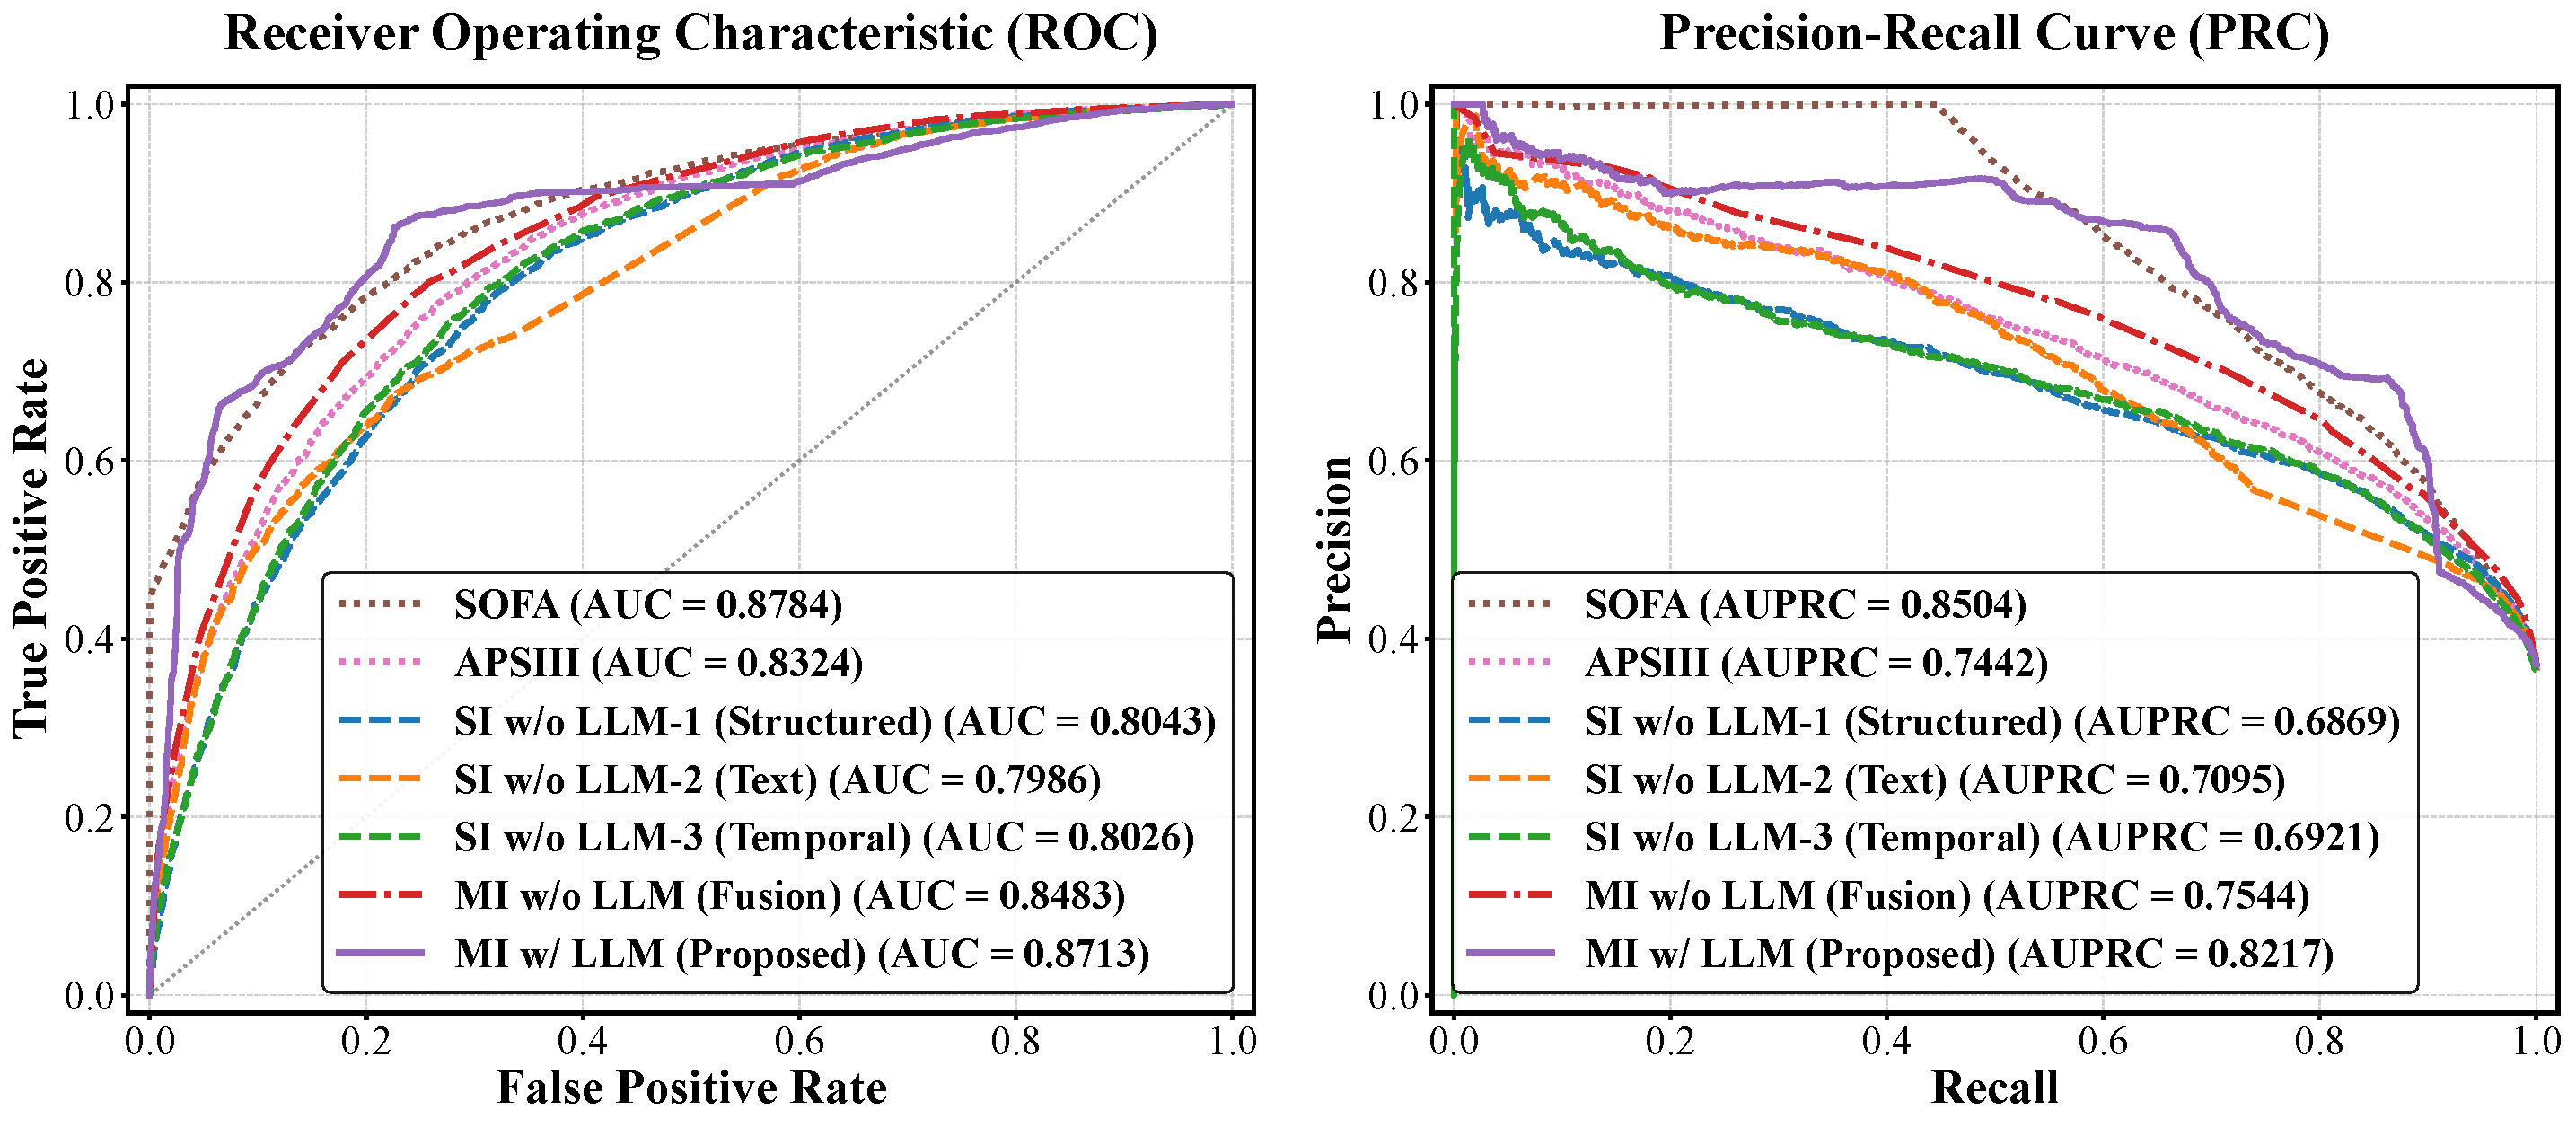
\includegraphics[width=0.95\linewidth]{figs/roc_pr_curves.pdf}
  \caption{ROC and PR curves comparing Cardio-Hybrid Net with traditional scores and single-modality baselines on the test set.The "SI w/o LLM-1", "SI w/o LLM-2", and "SI w/o LLM-3" baselines refer to the Struct.-only, Notes-only, and Time-series models, respectively.}
  \label{fig:roc-pr}
\end{figure}

\subsection{Ablation Studies on Model Design}

To balance computational efficiency and experimental depth, the ablation studies in this section are conducted on a representative subset ($N=5,000$) constructed via stratified sampling. While the reduced sample size yields absolute performance metrics slightly lower than those of the full model, it does not compromise the validity of verifying the relative trends across different architectural designs.

Table~\ref{tab:ablation} presents ablation studies on fusion strategy and attention design. Among all compared models, the tri-modal model utilizing the full attention mechanism (Full Attn) achieves the highest AUROC (0.8103), outperforming the Fixed-Wt Attn, Single-Layer Attn, and No-Cross Attn variants. This confirms that explicitly modeling cross-modal interactions is superior to simple concatenation, enabling the model to effectively capture complementary information across modalities \cite{Lyu2023MultimodalTransformer,XAI2023MultimodalICU}.

\begin{table}[t]
  \centering
  \small  % 核心：添加\small命令缩小字号（比默认\normalsize小一号）
  \caption{Ablation studies on Cardio-Hybrid Net model design.}
  \label{tab:ablation}

  \begin{tabular}{lcccc}
    \toprule
    \textbf{Model} & \textbf{AUROC} & \textbf{AUPRC}  \\
    \midrule
    Concat-Fuse (All Modalities) & 0.8099 & 0.7028 \\
    Single-Layer Attn (All Modalities) & 0.8040 & 0.6851 \\
    Struct-Only & 0.7681 & 0.6520 \\
    Struct+Temporal & 0.8085 & 0.6919 \\
    Struct+Text & 0.7791 & 0.6699 \\
    Temporal+Text & 0.7592 & 0.5858 \\
    Fixed-Wt Attn (All Modalities) & 0.8008 & 0.6628 \\
    No-Cross Attn (All Modalities) & 0.8035 & 0.6936 \\
    Full Attn (All Modalities) & \textbf{0.8103} & \textbf{0.6914} \\
    \bottomrule
  \end{tabular}
\end{table}

Furthermore, removing any single modality consistently leads to performance degradation. Notably, the exclusion of structural or temporal data results in significant drops, while the addition of textual information to the strong Struct+Temporal baseline yields further performance gains. These results underscore the necessity of tri-modal integration, where text narratives provide critical context that enhances the discriminative power of structured physiological signals.

\subsection{Effect of Uncertainty-Aware LLM Routing}

We evaluate the impact of uncertainty-aware LLM routing by comparing the base multi-attention model with the full Cardio-Hybrid Net in Table~\ref{tab:overall-performance}. The LLM-backed second stage consistently improves AUROC, AUPRC, and F1 scores. Sweeping the uncertainty threshold $\tau$ reveals a clear trade-off: lower thresholds mimic a high-cost ``always-call'' strategy, while increasing $\tau$ selectively targets ambiguous cases, preserving near-optimal performance with significantly reduced computational overhead.

As visualized in Figure~\ref{fig:Uncertainty Threshold and Interpretative Analysis}(a), our chosen operating point (vertical dashed line) routes approximately 30\% of patients to the LLM. This configuration recovers the majority of the performance gain (AUROC $\approx$ 0.86) while reducing LLM usage by two-thirds compared to the full-coverage approach. This efficiency is critical for deployment under resource constraints \cite{Griot2025LLMImplementationEHR,Du2024LLM_EHR_Survey}, allowing institutions to balance diagnostic precision with API and latency budgets.

\begin{figure*}[htbp!]
  \centering
  % Placeholder for threshold vs performance / call rate.

  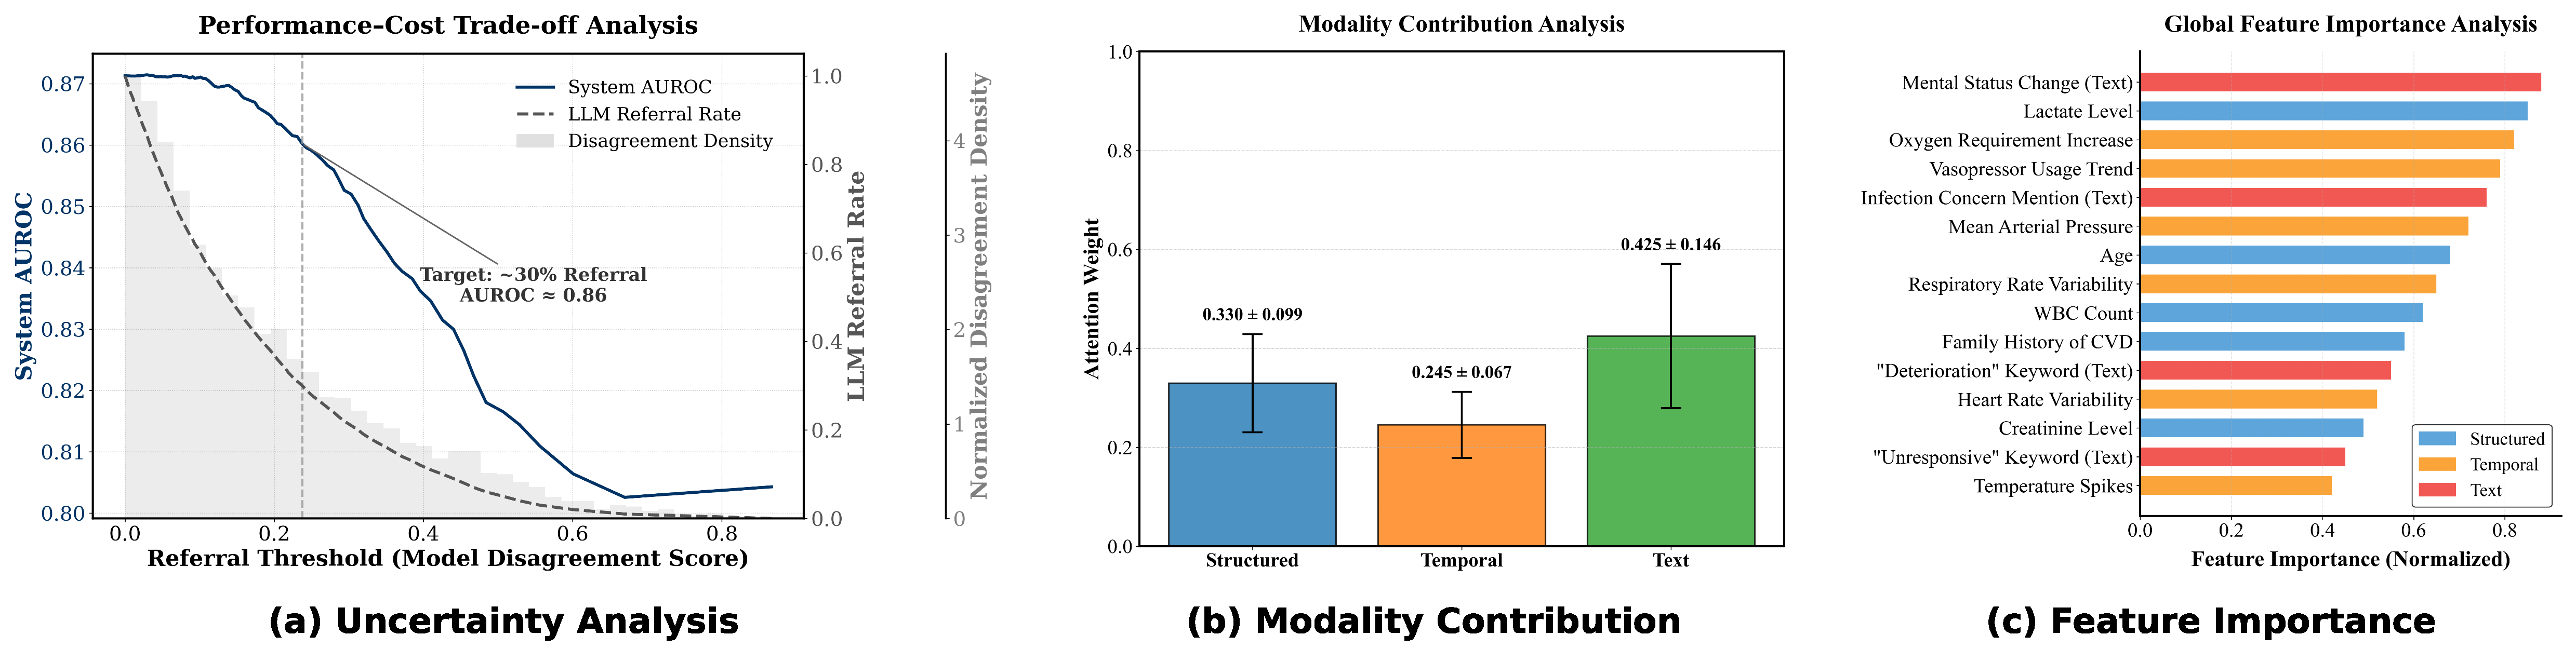
\includegraphics[width=0.95\linewidth]{figs/analysis.pdf}
  \caption{(a)Illustrative effect of the uncertainty threshold on AUROC and the fraction of patients routed to the LLM. (b)Model interpretability analysis. modality-level attention weights for structured, temporal, and textual inputs. (c)Model interpretability analysis. global feature importance across modalities.}
  \label{fig:Uncertainty Threshold and Interpretative Analysis}
\end{figure*}

Qualitatively, high-uncertainty cases often exhibit conflicting signals across modalities, such as stable vitals contradicting alarming clinical narratives. In these borderline scenarios, the LLM provides a semantic aggregation of multimodal evidence, effectively resolving ambiguities and aligning the predicted risk closer to the true clinical outcome.

\subsection{Interpretability and Case Studies}

We analyze modality-level attention weights and feature importance scores to understand how Cardio-Hybrid Net makes decisions, following recent work on explainable multimodal ICU models \cite{XAI2023MultimodalICU}.

As illustrated in Figure~\ref{fig:Uncertainty Threshold and Interpretative Analysis}(b)and(c), the model exhibits a clear hierarchical preference for unstructured data. The \textit{Textual Modality} commands the highest average attention weight ($0.425 \pm 0.146$), significantly surpassing structured ($0.330 \pm 0.099$) and temporal ($0.245 \pm 0.067$) modalities. This macro-level dominance is corroborated by granular feature importance analysis, where \textit{``Mental Status Change''} (textual) emerges as the top predictor. This is complemented by critical physiological indicators such as \textit{``Lactate Level''} (structured) and \textit{``Vasopressor Usage Trend''} (temporal). These findings challenge the traditional reliance on numerical vitals alone, suggesting that the model successfully integrates high-level semantic narratives with objective physiological markers to capture the multifaceted nature of hemodynamic instability.

We also examine per-patient attention maps and retrieved similar cases for representative examples.(\textit{See the attached page.})

\section{Discussion}

Our results suggest that LLMs are most valuable in ICU risk prediction when used as conditional consultants rather than universal predictors.
By building on a strong multimodal base model and invoking the LLM only for uncertain cases, Cardio-Hybrid Net achieves a favorable balance between predictive performance and computational cost \cite{Gal2016DropoutUncertainty,Griot2025LLMImplementationEHR,Lin2025LLMHealthcareRoles}.

Compared with prior multimodal ICU models that simply fuse time series and notes \cite{Khadanga2019ICUNotes,Shukla2020IntegratingTSNotes,Lyu2023MultimodalTransformer}, our framework explicitly models when LLM assistance is needed, which mirrors clinical practice where physicians seek additional consultation only in ambiguous or high-risk scenarios.
From a methodological perspective, our findings emphasize the importance of uncertainty-aware routing, well-designed prompts, and careful calibration when integrating LLMs into structured prediction pipelines \cite{Lewis2020RAG,Geifman2017SelectiveClassification,Moons2015TRIPOD}.

\subsection{Clinical and Workflow Implications}

From a clinical perspective, our findings support a layered decision-support architecture: a calibrated, interpretable local model for the majority of patients, and an LLM-backed second opinion for difficult cases.
In a typical deployment, the risk score and short textual rationale produced by the system could be surfaced within the ICU electronic record, with clear distinction between data-driven risk estimates and generated explanations.
The clinician remains the ultimate decision-maker, with the hybrid model acting primarily as a triage and prioritization tool rather than a replacement for clinical judgment \cite{Griot2025LLMImplementationEHR,Du2024LLM_EHR_Survey}.

The ability to control the routing threshold provides a practical knob to adapt the system to local resource constraints: units with limited compute or network connectivity might operate at higher thresholds, using the LLM only for the most ambiguous cases, whereas tertiary centers with stronger infrastructure could afford more frequent LLM consultation.
In all scenarios, clear communication of model confidence and the provenance of explanations is crucial to maintain trust and avoid overreliance.

\subsection{Methodological Perspective and Generalization}

From a methodological perspective, Cardio-Hybrid Net can be viewed as an instance of a broader pattern: combining a structured predictor that is well calibrated on the data distribution with a flexible, knowledge-rich but expensive expert that is consulted selectively \cite{Gal2016DropoutUncertainty,Geifman2017SelectiveClassification}.
In our case the expert is an LLM; in other domains it could be a human clinician, a treatment guideline engine, or a specialized physics-based simulator.

The same architecture can be adapted to other high-risk prediction tasks such as sepsis, respiratory failure, or neurological deterioration \cite{OzrazgatBaslanti2021AIICU,Hyland2020HiRID}.
As long as multimodal EHR data are available, a tri-stream encoder with cross-modal attention can serve as a base model, and uncertainty-aware routing can be applied to decide when to query an external expert model.
This provides a useful abstraction for designing future AI systems in healthcare and other safety-critical domains.

\subsection{Limitations and Future Work}

This study has several limitations.
First, it relies on a single large academic center dataset (MIMIC-IV); external validation on independent cohorts such as eICU and HiRID is needed to assess generalizability across institutions and practice patterns \cite{Pollard2018eICU,Hyland2020HiRID}.
Second, although we incorporated uncertainty estimates via Monte Carlo dropout, we did not systematically compare alternative uncertainty quantification methods (e.g., deep ensembles or conformal methods) that might further improve selective prediction \cite{Gal2016DropoutUncertainty}.

Third, while our RAG pipeline grounds LLM inputs in structured EHR data and retrieved similar cases, we did not perform a detailed ablation over different prompt designs, retrieval strategies, or LLM families \cite{Lewis2020RAG,Du2024LLM_EHR_Survey}.
Finally, regulatory, ethical, and workflow considerations---including data privacy, bias, and human-factor engineering---must be carefully addressed before deploying such systems in real ICUs \cite{Lin2025LLMHealthcareRoles,Loh2018AIRole}.

Future work will investigate more sophisticated meta-routers that consider not only uncertainty but also patient-level context and resource constraints, and extend the framework to other high-risk prediction tasks and clinical settings.
Prospective evaluations and user studies with clinicians will be crucial for understanding how hybrid LLM--EHR systems affect clinical decision-making, workload, and patient outcomes.

\section{Conclusion}

We presented Cardio-Hybrid Net, an uncertainty-aware, LLM-guided multimodal framework for early prediction of cardiovascular deterioration in the ICU.
By combining structured data, time series, and clinical notes with selective LLM consultation, our approach improves predictive performance over both traditional scores and strong multimodal baselines, while using the LLM only when it is most needed.
\section*{Ethics Statement}
This study uses only de-identified, publicly available ICU data (MIMIC-IV) and does not involve any direct patient contact or intervention.
We follow the data usage agreement of the MIMIC project and discuss the potential risks of miscalibration and automation bias when deploying hybrid LLM--EHR models in clinical workflows.

\bibliographystyle{named}
\bibliography{refs}


\end{document}
